\chapter{Implementacija i korisničko sučelje}
		
		
		\section{Korištene tehnologije i alati}
		
			\textbf{\textit{dio 2. revizije}}
			
			Komunikacija među članovima tima realizirana je korištenjem aplikacija WhatsApp\footnote{\href{https://www.whatsapp.com/}{https://www.whatsapp.com/}} i Discord\footnote{\href{https://discord.com/}{https://discord.com/}}. Za izradu sekvencijskih dijagrama korišten je web alat za izradu dijagrama Online Visual Paradigm\footnote{\href{https://online.visual-paradigm.com/}{https://online.visual-paradigm.com/}}. Za izradu svih ostalih dijagrama korišten je program Astah\footnote{\href{https://astah.net/}{https://astah.net/}} koji služi za modeliranje i izradu dijagrama u inženjerskoj struci.
			
			Upravljanje izvornim kodom ostvareno je korištenjem sustava Git\footnote{\href{https://git-scm.com/}{https://git-scm.com/}}, a udaljeni repozitorij projekta dostupan je na web sustavu GitLab\footnote{\href{https://about.gitlab.com/}{https://about.gitlab.com/}}.\\
			
			Frontend aplikacije napravljen je u razvojnom okruženju Android Studio\footnote{\href{https://developer.android.com/studio?gclid=CjwKCAiA24SPBhB0EiwAjBgkhjQMRvsHMZCuxfC4b_03_6rtMeVgpqzEHRJTu-w7eo0ddFUCdb-aWBoC-C8QAvD_BwE&gclsrc=aw.ds}{Android Studio}} koristeći programski jezik Java\footnote{\href{https://www.java.com/en/}{https://www.java.com/en/}}. Android Studio je službeno razvojno okruženje za Android platformu i temelji se na InteliJ IDEA-u. Prvenstveno se koristi za izradu Android aplikacija i igara. Pri razvoju softvera Android Studio koristi Gradle tehnologiju, predloške koda s GitHub-a i podršku za korištenje Google Cloud platforme.\\ 
			
			Backend aplikacije je napisan programskim jezikom Python\footnote{\href{https://www.python.org/}{https://www.python.org/}} u razvojnom okruženju Visual Studio Code\footnote{\href{https://code.visualstudio.com/}{https://code.visualstudio.com/}}. Visual Studio Code se najviše koristi za pisanje i debbugiranje programskog koda aplikacija. Uz standardne funkcionalnosti Pythona korišten je i adapter za komunikaciju s bazom podataka Psycopg2\footnote{\href{https://pypi.org/project/psycopg2/}{https://pypi.org/project/psycopg2/}}.\\
			
			Dodatno je za ostvarenje backenda korištena i cloud platforma Amazon AWS\footnote{\href{https://aws.amazon.com}{Amazon AWS}}. Konkretno su korištene usluge AWS Lambda\footnote{\href{https://aws.amazon.com/lambda/?nc2=h\_ql\_prod\_fs\_lbd}{https://aws.amazon.com/lambda/?nc2=h\_ql\_prod\_fs\_lbd}}, API Gateway\footnote{\href{https://aws.amazon.com/api-gateway/?nc2=type\_a}{https://aws.amazon.com/api-gateway/?nc2=type\_a}} i RDS Database\footnote{\href{https://aws.amazon.com/rds/?nc2=type\_a}{https://aws.amazon.com/rds/?nc2=type\_a}}. API Gateway služi za preusmjeravanje HTTP zahtjeva s frontenda na AWS Lambdu u kojoj su implementirane funkcionalnosti backenda. AWS Lambda zatim preko istog API Gatewaya šalje odgovor frontendu. \\
			
			Baza podataka nalazi se na poslužitelju Amazon RDS.
			
			\eject 
		
	
		\section{Ispitivanje programskog rješenja}
			
			\textbf{\textit{dio 2. revizije}}\\
			
			
	
			
			\subsection{Ispitivanje komponenti}
			
			\textbf{Ispitni slučaj 1: Registracija novog korisnika}\\
			\begin{itemize}
				\item funkciji register\_handler predaju se podaci o korsiniku u JSON formatu
				\item funkcija stvara element klase User i poziva metodu register
			
			\item očekivani rezultat:\\
				\begin{itemize}
					\item funkcija vraća poruku "SignupValid" 
					\item korisnik se upisuje u bazu podataka
				\end{itemize}
			\item rezultat:
		\end{itemize}
			\begin{figure}[H]
				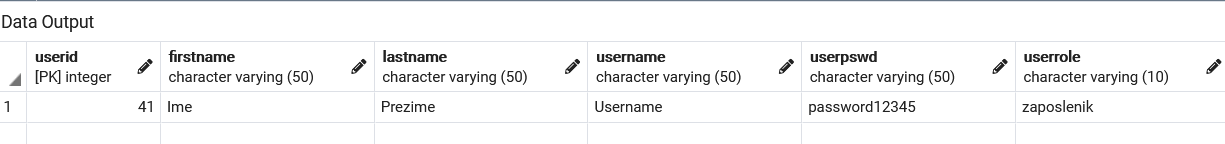
\includegraphics[scale=0.5]{./slike/baza1.png}
				\caption{Rezultat u bazi podataka}
				\label{fig:REZ1}
			\end{figure}

			\begin{figure}[H]
				\centering
				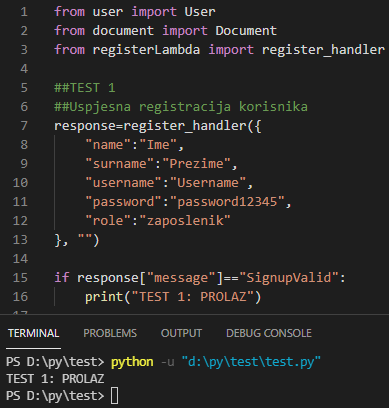
\includegraphics[scale=0.5]{./slike/rez1.png}
				\caption{Rezultat u razvojnom okruženju}
				\label{fig:REZ1}
			\end{figure}
		
		
		\textbf{Ispitni slučaj 2: Pokušaj registracije s već postojećim korisničkim imenom:}\\
		\begin{itemize}
			\item funkciji register\_handler predaju se podaci o korsiniku u JSON formatu
			\item funkcija stvara element klase User i poziva metodu register
			
			\item očekivani rezultat:\\
			\begin{itemize}
				\item funkcija vraća poruku "SignupInvalid" 
				\item korisnik se ne upisuje u bazu podataka
			\end{itemize}
			\item rezultat:
		\end{itemize}
		\begin{figure}[H]
			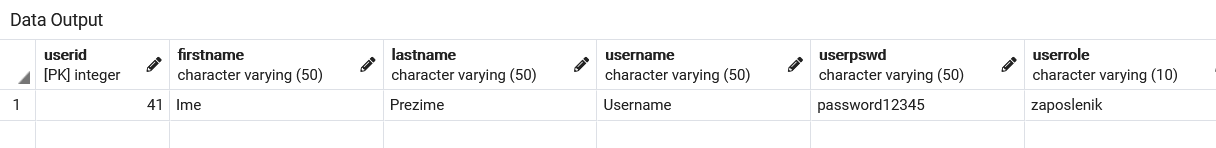
\includegraphics[scale=0.5]{./slike/baza2.png}
			\caption{Potvrda rezultata u bazi podataka}
			\label{fig:REZ2}
		\end{figure}
		
		\begin{figure}[H]
			\centering
			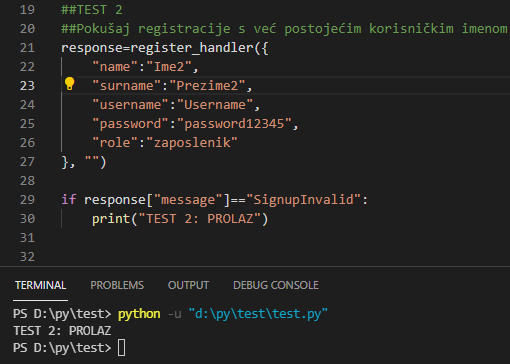
\includegraphics[scale=0.5]{./slike/rez2.png}
			\caption{Rezultat u razvojnom okruženju}
			\label{fig:REZ2}
		\end{figure}
	
	
		\textbf{Ispitni slučaj 3: Login postojećeg korisnika:}\\
\begin{itemize}
	\item funkciji login\_handler predaju se podaci o korsiniku u JSON formatu
	\item funkcija dohvaća korisnika iz baze koristeći korisničko ime
	
	\item očekivani rezultat:\\
	\begin{itemize}
		\item funkcija vraća poruku "LoginValid" 
		\item uz poruku vraća i podatke o korisniku
	\end{itemize}
	\item rezultat:
\end{itemize}
\begin{figure}[H]
	\centering
	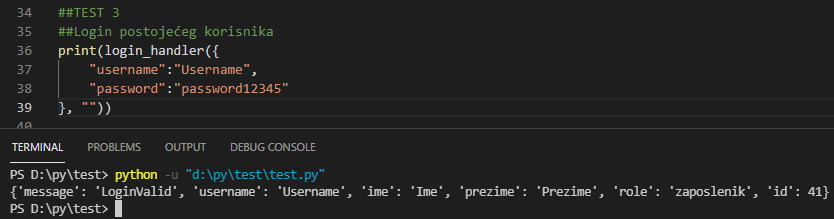
\includegraphics[scale=0.5]{./slike/rez3.png}
	\caption{Rezultat u razvojnom okruženju}
	\label{fig:REZ3}
\end{figure}


		\textbf{Ispitni slučaj 4: Login nepostojećeg korisnika:}\\
\begin{itemize}
	\item funkciji login\_handler predaju se podaci o korsiniku u JSON formatu
	\item funkcija pokušava dohvatiti korisnika iz baze koristeći korisničko ime
	
	\item očekivani rezultat:\\
	\begin{itemize}
		\item funkcija vraća poruku "LoginInvalid" 
		\item uz poruku vraća i prazne podatke o korisniku
	\end{itemize}
	\item rezultat:
\end{itemize}
\begin{figure}[H]
	\centering
	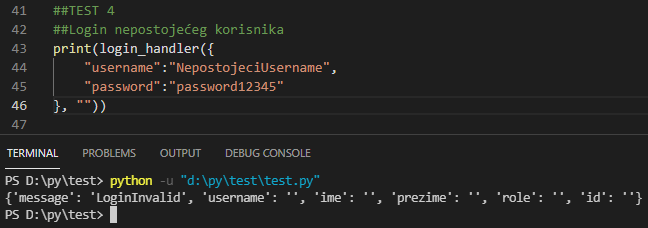
\includegraphics[scale=0.5]{./slike/rez4.png}
	\caption{Rezultat u razvojnom okruženju}
	\label{fig:REZ4}
\end{figure}


		\textbf{Ispitni slučaj 5: Pokušaj logina postojećeg korisnika s neispravnom lozinkom:}\\
\begin{itemize}
	\item funkciji login\_handler predaju se podaci o korsiniku u JSON formatu
	\item funkcija dohvaća korisnika iz baze podataka koristeći korisničko ime i uspoređuje lozinke 
	
	\item očekivani rezultat:\\
	\begin{itemize}
		\item funkcija vraća poruku "LoginInvalid" 
		\item uz poruku vraća i podatke o korisniku jer korisnik postoji, samo je lozinka neispravna
	\end{itemize}
	\item rezultat:
\end{itemize}
\begin{figure}[H]
	\centering
	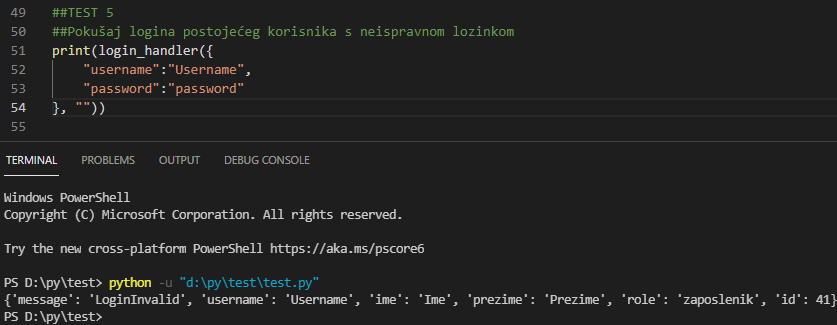
\includegraphics[scale=0.5]{./slike/rez5.png}
	\caption{Rezultat u razvojnom okruženju}
	\label{fig:REZ5}
\end{figure}


		\textbf{Ispitni slučaj 6: Dodavanje ispravno skeniranog dokumenta:}\\
\begin{itemize}
	\item funkciji add\_document\_handler predaju se podaci o dokumentu, datum skeniranja i ID korisnika koji je skenirao dokument
	\item funkcija stvara objekt klase Document i poziva metodu addDocument
	\item funkcija addDocument dodaje zapis o skeniranju u relacije "scanhistory", "documents" i, ako je dokument označen kao ispravan, u relaciju "reviserpending" ili "accountantpending" 
	
	\item očekivani rezultat:\\
	\begin{itemize}
		\item funkcija dodaje zapise o skeniranju dokumenta u relacije "scanhistory", "documents" i, pošto je korisnik koji je skenirao dokument zaposlenik, u relaciju "reviserpending"
	\end{itemize}
	\item rezultat:
\end{itemize}
\begin{figure}[H]
	\centering
	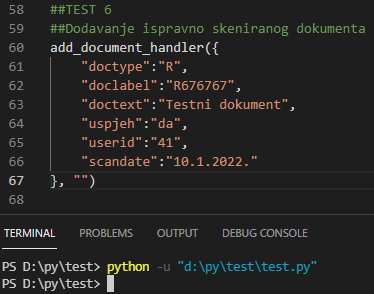
\includegraphics[scale=0.5]{./slike/rez6.png}
	\caption{Rezultat u razvojnom okruženju}
	\label{fig:REZ6}
\end{figure}
\begin{figure}[H]
	\centering
	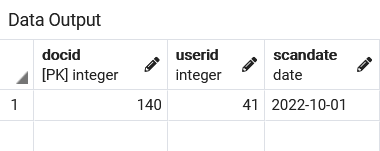
\includegraphics[scale=0.5]{./slike/baza6sh.png}
	\caption{Rezultat u relaciji "scanhistory"}
	\label{fig:BAZA6a}
\end{figure}
\begin{figure}[H]
	\centering
	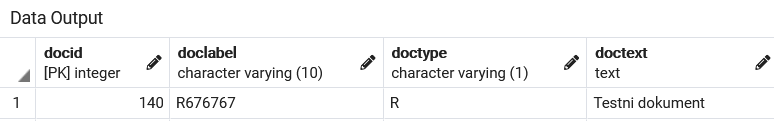
\includegraphics[scale=0.5]{./slike/baza6doc.png}
	\caption{Rezultat u relaciji "documents"}
	\label{fig:BAZA6b}
\end{figure}
\begin{figure}[H]
	\centering
	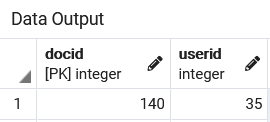
\includegraphics[scale=0.5]{./slike/baza6rp.png}
	\caption{Rezultat u relaciji "reviserpending"}
	\label{fig:BAZA6c}
\end{figure}


		\textbf{Ispitni slučaj 7: Dodavanje neispravno skeniranog dokumenta:}\\
\begin{itemize}
	\item funkciji add\_document\_handler predaju se podaci o dokumentu, datum skeniranja i ID korisnika koji je skenirao dokument
	\item funkcija stvara objekt klase Document i poziva metodu addDocument
	\item funkcija addDocument dodaje zapis o skeniranju u relacije "scanhistory", "documents" i, ako je dokument označen kao ispravan, u relaciju "reviserpending" ili "accountantpending" 
	
	\item očekivani rezultat:\\
	\begin{itemize}
		\item funkcija dodaje zapise o skeniranju dokumenta u relacije "scanhistory", "documents" i, pošto je dokument označen kao pogrešno skeniran, ne dodaje ga u relaciju "reviserpending"
	\end{itemize}
	\item rezultat:
	\begin{itemize}
		\item funkcija je prošla test
	\end{itemize}
\end{itemize}
\begin{figure}[H]
	\centering
	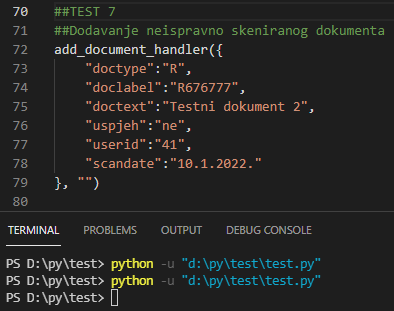
\includegraphics[scale=0.5]{./slike/rez7.png}
	\caption{Rezultat u razvojnom okruženju}
	\label{fig:REZ7}
\end{figure}
\begin{figure}[H]
	\centering
	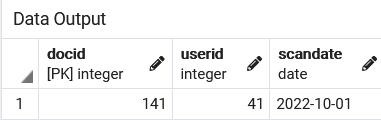
\includegraphics[scale=0.5]{./slike/baza7sh.png}
	\caption{Rezultat u relaciji "scanhistory"}
	\label{fig:BAZA7a}
\end{figure}
\begin{figure}[H]
	\centering
	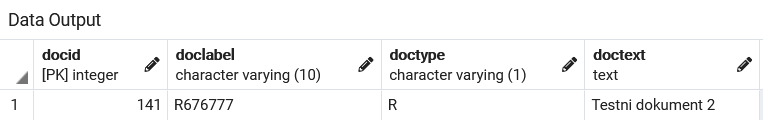
\includegraphics[scale=0.5]{./slike/baza7doc.png}
	\caption{Rezultat u relaciji "documents"}
	\label{fig:BAZA7b}
\end{figure}
\begin{figure}[H]
	\centering
	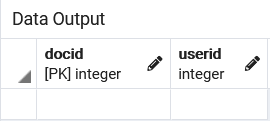
\includegraphics[scale=0.5]{./slike/baza7rp.png}
	\caption{Rezultat u relaciji "reviserpending"}
	\label{fig:BAZA7c}
\end{figure}


	\textbf{Ispitni slučaj 8: Slučajno dodavanje dokumenta kao ispravnog iako je oznaka dokumenta pogrešno skenirana:}\\
\begin{itemize}
	\item funkciji add\_document\_handler predaju se podaci o dokumentu, datum skeniranja i ID korisnika koji je skenirao dokument
	\item funkcija stvara objekt klase Document i poziva metodu addDocument
	\item funkcija addDocument dodaje zapis o skeniranju u relacije "scanhistory", "documents" i, ako je dokument označen kao ispravan, u relaciju "reviserpending" ili "accountantpending"
	\item pošto je oznaka dokumenta pogrešno skenirana, frontend aplikacije backendu šalje prazan string kao atribut "doclabel"
	
	\item očekivani rezultat:\\
	\begin{itemize}
		\item funkcija dodaje zapise o skeniranju dokumenta u relacije "scanhistory", "documents" i, unatoč tome što je dokument označen kao ispravno skeniran, ne dodaje ga u relaciju "reviserpending" jer je "doclabel" prazan string
		\item vrijednosti "doclabel" i "doctype" su u relaciji document postavljene kao null vrijednosti
	\end{itemize}
	\item rezultat:
	\begin{itemize}
		\item funkcija je prošla test
	\end{itemize}
\end{itemize}
\begin{figure}[H]
	\centering
	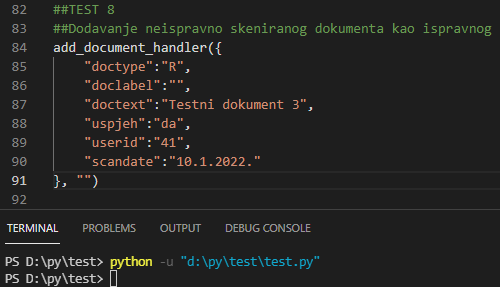
\includegraphics[scale=0.5]{./slike/rez8.png}
	\caption{Rezultat u razvojnom okruženju}
	\label{fig:REZ8}
\end{figure}
\begin{figure}[H]
	\centering
	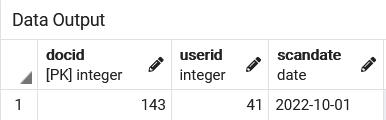
\includegraphics[scale=0.5]{./slike/baza8sh.png}
	\caption{Rezultat u relaciji "scanhistory"}
	\label{fig:BAZA8a}
\end{figure}
\begin{figure}[H]
	\centering
	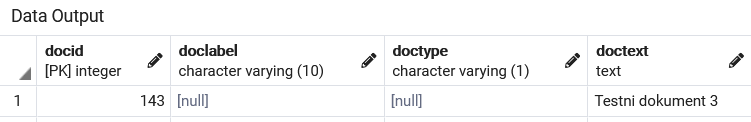
\includegraphics[scale=0.5]{./slike/baza8doc.png}
	\caption{Rezultat u relaciji "documents"}
	\label{fig:BAZA8b}
\end{figure}
\begin{figure}[H]
	\centering
	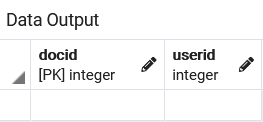
\includegraphics[scale=0.5]{./slike/baza8rp.png}
	\caption{Rezultat u relaciji "reviserpending"}
	\label{fig:BAZA8c}
\end{figure}
			
		
			
			\subsection{Ispitivanje sustava}
			\subsubsection{Testiranje logina}
			Testiramo može li se korisnik prijaviti u aplikaciju.
			\begin{lstlisting}[language=Java]
				@LargeTest
				@RunWith(AndroidJUnit4.class)
				public class login_radnik_test {
					
					@Rule
					public ActivityTestRule<MainActivity> mActivityTestRule = new ActivityTestRule<>(MainActivity.class);
					
					@Test
					public void login_radnik_test() {
						ViewInteraction appCompatEditText = onView(
						allOf(withId(R.id.etUsername),
						childAtPosition(
						allOf(withId(R.id.LogInText),
						childAtPosition(
						withId(android.R.id.content),
						0)),
						1),
						isDisplayed()));
						appCompatEditText.perform(replaceText("radnik"), closeSoftKeyboard());
						
						ViewInteraction appCompatEditText2 = onView(
						allOf(withId(R.id.etPassword),
						childAtPosition(
						allOf(withId(R.id.LogInText),
						childAtPosition(
						withId(android.R.id.content),
						0)),
						2),
						isDisplayed()));
						appCompatEditText2.perform(replaceText("rad1234"), closeSoftKeyboard());
						
						ViewInteraction appCompatEditText3 = onView(
						allOf(withId(R.id.etPassword), withText("rad1234"),
						childAtPosition(
						allOf(withId(R.id.LogInText),
						childAtPosition(
						withId(android.R.id.content),
						0)),
						2),
						isDisplayed()));
						appCompatEditText3.perform(pressImeActionButton());
						
						ViewInteraction materialButton = onView(
						allOf(withId(R.id.LoginBtn), withText("Log In"),
						childAtPosition(
						allOf(withId(R.id.LogInText),
						childAtPosition(
						withId(android.R.id.content),
						0)),
						3),
						isDisplayed()));
						materialButton.perform(click());
					}
					
					private static Matcher<View> childAtPosition(
					final Matcher<View> parentMatcher, final int position) {
						
						return new TypeSafeMatcher<View>() {
							@Override
							public void describeTo(Description description) {
								description.appendText("Child at position " + position + " in parent ");
								parentMatcher.describeTo(description);
							}
							
							@Override
							public boolean matchesSafely(View view) {
								ViewParent parent = view.getParent();
								return parent instanceof ViewGroup && parentMatcher.matches(parent)
								&& view.equals(((ViewGroup) parent).getChildAt(position));
							}
						};
					}
				}
			\end{lstlisting}
		
		Ako je login ispravan, proći ćemo test.
		
		\begin{figure}[H]
			\centering
			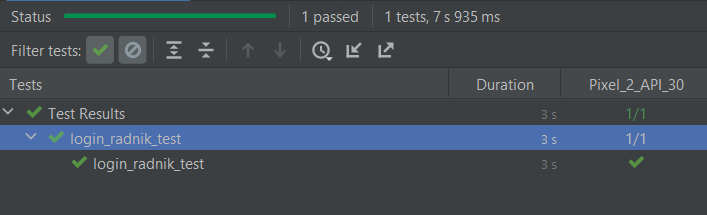
\includegraphics[scale=0.5]{./slike/test1.png}
			\caption{"Test logina"}
			\label{fig:test1}
		\end{figure}\eject
	
		\subsubsection{Testiranje prisutnosti slike u ImageView-u}
	Testiramo je li slika prisutna u ImageView-u.
	\begin{lstlisting}[language=Java]
	@LargeTest
	@RunWith(AndroidJUnit4.class)
	public class prikazuje_sliku_test {
		
		@Rule
		public ActivityTestRule<MainActivity> mActivityTestRule = new ActivityTestRule<>(MainActivity.class);
		
		@Rule
		public GrantPermissionRule mGrantPermissionRule =
		GrantPermissionRule.grant(
		"android.permission.CAMERA");
		
		@Test
		public void prikazuje_sliku_test() {
			ViewInteraction appCompatEditText = onView(
			allOf(withId(R.id.etUsername),
			childAtPosition(
			allOf(withId(R.id.LogInText),
			childAtPosition(
			withId(android.R.id.content),
			0)),
			1),
			isDisplayed()));
			appCompatEditText.perform(replaceText("radnik"), closeSoftKeyboard());
			
			ViewInteraction appCompatEditText2 = onView(
			allOf(withId(R.id.etPassword),
			childAtPosition(
			allOf(withId(R.id.LogInText),
			childAtPosition(
			withId(android.R.id.content),
			0)),
			2),
			isDisplayed()));
			appCompatEditText2.perform(replaceText("rad1234"), closeSoftKeyboard());
			
			ViewInteraction materialButton = onView(
			allOf(withId(R.id.LoginBtn), withText("Log In"),
			childAtPosition(
			allOf(withId(R.id.LogInText),
			childAtPosition(
			withId(android.R.id.content),
			0)),
			3),
			isDisplayed()));
			materialButton.perform(click());
			
			ViewInteraction materialButton2 = onView(
			allOf(withId(R.id.ScanZap), withText("Skeniranje"),
			childAtPosition(
			childAtPosition(
			withId(android.R.id.content),
			0),
			0),
			isDisplayed()));
			materialButton2.perform(click());
			
			try {
				TimeUnit.SECONDS.sleep(2);
			} catch (InterruptedException e) {
				e.printStackTrace();
			}
			
			ViewInteraction materialButton3 = onView(withId(R.id.SlikajButton));
			materialButton3.perform(click());
			try {
				TimeUnit.SECONDS.sleep(2);
			} catch (InterruptedException e) {
				e.printStackTrace();
			}
			onView(withId(R.id.SlikaWind)).check(matches(notNullValue()));
		}
		
		private static Matcher<View> childAtPosition(
		final Matcher<View> parentMatcher, final int position) {
			
			return new TypeSafeMatcher<View>() {
				@Override
				public void describeTo(Description description) {
					description.appendText("Child at position " + position + " in parent ");
					parentMatcher.describeTo(description);
				}
				
				@Override
				public boolean matchesSafely(View view) {
					ViewParent parent = view.getParent();
					return parent instanceof ViewGroup && parentMatcher.matches(parent)
					&& view.equals(((ViewGroup) parent).getChildAt(position));
				}
			};
		}
	}
	\end{lstlisting}
	
	Ako je slika u ImageView-u, proći ćemo test.
	
	\begin{figure}[H]
		\centering
		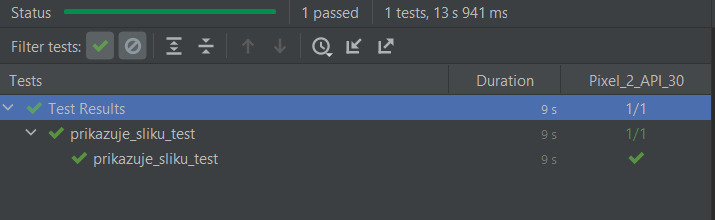
\includegraphics[scale=0.5]{./slike/test2.png}
		\caption{"Test prisutnosti slike u ImageView-u"}
		\label{fig:test2}
	\end{figure}\eject


	\subsubsection{Testiranje ispravnog skena dokumenta}
Testiramo je li skenirani dokument ispravan.
Ispravan dokument je:\\
Internal file in our app\\
INT9852
\begin{lstlisting}[language=Java]
@LargeTest
@RunWith(AndroidJUnit4.class)
public class ispravanSkenTest {
	
	@Rule
	public ActivityTestRule<MainActivity> mActivityTestRule = new ActivityTestRule<>(MainActivity.class);
	
	@Rule
	public GrantPermissionRule mGrantPermissionRule =
	GrantPermissionRule.grant(
	"android.permission.CAMERA");
	
	@Test
	public void ispravanSkenTest() {
		ViewInteraction appCompatEditText = onView(
		allOf(withId(R.id.etUsername),
		childAtPosition(
		allOf(withId(R.id.LogInText),
		childAtPosition(
		withId(android.R.id.content),
		0)),
		1),
		isDisplayed()));
		appCompatEditText.perform(replaceText("user12"), closeSoftKeyboard());
		
		ViewInteraction appCompatEditText2 = onView(
		allOf(withId(R.id.etPassword),
		childAtPosition(
		allOf(withId(R.id.LogInText),
		childAtPosition(
		withId(android.R.id.content),
		0)),
		2),
		isDisplayed()));
		appCompatEditText2.perform(replaceText("user12"), closeSoftKeyboard());
		
		ViewInteraction materialButton = onView(
		allOf(withId(R.id.LoginBtn), withText("Log In"),
		childAtPosition(
		allOf(withId(R.id.LogInText),
		childAtPosition(
		withId(android.R.id.content),
		0)),
		3),
		isDisplayed()));
		materialButton.perform(click());
		
		ViewInteraction materialButton2 = onView(
		allOf(withId(R.id.ScanZap), withText("Skeniranje"),
		childAtPosition(
		childAtPosition(
		withId(android.R.id.content),
		0),
		0),
		isDisplayed()));
		materialButton2.perform(click());
		try {
			TimeUnit.SECONDS.sleep(10);
		} catch (InterruptedException e) {
			e.printStackTrace();
		}
		ViewInteraction materialButton3 = onView(
		allOf(withId(R.id.SlikajButton), withText("SLIKAJ"),
		childAtPosition(
		childAtPosition(
		withId(android.R.id.content),
		0),
		1),
		isDisplayed()));
		materialButton3.perform(click());
		try {
			TimeUnit.SECONDS.sleep(3);
		} catch (InterruptedException e) {
			e.printStackTrace();
		}
		
		ViewInteraction materialButton4 = onView(
		allOf(withId(R.id.SkenirajSlikuButton), withText("Skeniraj Sliku"),
		childAtPosition(
		childAtPosition(
		withId(android.R.id.content),
		0),
		2),
		isDisplayed()));
		materialButton4.perform(click());
		try {
			TimeUnit.SECONDS.sleep(3);
		} catch (InterruptedException e) {
			e.printStackTrace();
		}
		ViewInteraction textView = onView(
		allOf(withId(R.id.SkeniraniTekst),
		withParent(withParent(withId(android.R.id.content))),
		isDisplayed()));
		textView.check(matches(withText("Internal file in our app\nINT9852\n")));
		try {
			TimeUnit.SECONDS.sleep(3);
		} catch (InterruptedException e) {
			e.printStackTrace();
		}
		ViewInteraction materialButton5 = onView(
		allOf(withId(R.id.IspravanScanButton), withText("Ispravan Scan"),
		childAtPosition(
		childAtPosition(
		withId(android.R.id.content),
		0),
		1),
		isDisplayed()));
		materialButton5.perform(click());
		try {
			TimeUnit.SECONDS.sleep(3);
		} catch (InterruptedException e) {
			e.printStackTrace();
		}
	}
	
	private static Matcher<View> childAtPosition(
	final Matcher<View> parentMatcher, final int position) {
		
		return new TypeSafeMatcher<View>() {
			@Override
			public void describeTo(Description description) {
				description.appendText("Child at position " + position + " in parent ");
				parentMatcher.describeTo(description);
			}
			
			@Override
			public boolean matchesSafely(View view) {
				ViewParent parent = view.getParent();
				return parent instanceof ViewGroup && parentMatcher.matches(parent)
				&& view.equals(((ViewGroup) parent).getChildAt(position));
			}
		};
	}
}

\end{lstlisting}

Ako je skenirani dokument ispravan, proći ćemo test.

\begin{figure}[H]
	\centering
	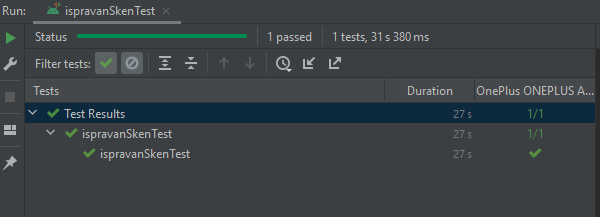
\includegraphics[scale=1]{./slike/test3.png}
	\caption{"Test ispravnosti skeniranog dokumenta"}
	\label{fig:test3}
\end{figure}\eject


	\subsubsection{Testiranje neispravnog skena dokumenta}
Testiramo je li skenirani dokument neispravan.
Ispravan dokument je:\\
Internal file in our app\\
INT9852
\begin{lstlisting}[language=Java]
	@LargeTest
	@RunWith(AndroidJUnit4.class)
	public class neispravanSkenTest {
		
		@Rule
		public ActivityTestRule<MainActivity> mActivityTestRule = new ActivityTestRule<>(MainActivity.class);
		
		@Rule
		public GrantPermissionRule mGrantPermissionRule =
		GrantPermissionRule.grant(
		"android.permission.CAMERA");
		
		@Test
		public void neispravanSkenTest() {
			ViewInteraction appCompatEditText = onView(
			allOf(withId(R.id.etUsername),
			childAtPosition(
			allOf(withId(R.id.LogInText),
			childAtPosition(
			withId(android.R.id.content),
			0)),
			1),
			isDisplayed()));
			appCompatEditText.perform(replaceText("user12"), closeSoftKeyboard());
			
			ViewInteraction appCompatEditText2 = onView(
			allOf(withId(R.id.etPassword),
			childAtPosition(
			allOf(withId(R.id.LogInText),
			childAtPosition(
			withId(android.R.id.content),
			0)),
			2),
			isDisplayed()));
			appCompatEditText2.perform(replaceText("user12"), closeSoftKeyboard());
			
			ViewInteraction appCompatEditText3 = onView(
			allOf(withId(R.id.etPassword), withText("user12"),
			childAtPosition(
			allOf(withId(R.id.LogInText),
			childAtPosition(
			withId(android.R.id.content),
			0)),
			2),
			isDisplayed()));
			appCompatEditText3.perform(pressImeActionButton());
			
			ViewInteraction materialButton = onView(
			allOf(withId(R.id.LoginBtn), withText("Log In"),
			childAtPosition(
			allOf(withId(R.id.LogInText),
			childAtPosition(
			withId(android.R.id.content),
			0)),
			3),
			isDisplayed()));
			materialButton.perform(click());
			
			ViewInteraction materialButton2 = onView(
			allOf(withId(R.id.ScanZap), withText("Skeniranje"),
			childAtPosition(
			childAtPosition(
			withId(android.R.id.content),
			0),
			0),
			isDisplayed()));
			materialButton2.perform(click());
			try {
				TimeUnit.SECONDS.sleep(10);
			} catch (InterruptedException e) {
				e.printStackTrace();
			}
			ViewInteraction materialButton3 = onView(
			allOf(withId(R.id.SlikajButton), withText("SLIKAJ"),
			childAtPosition(
			childAtPosition(
			withId(android.R.id.content),
			0),
			1),
			isDisplayed()));
			materialButton3.perform(click());
			try {
				TimeUnit.SECONDS.sleep(3);
			} catch (InterruptedException e) {
				e.printStackTrace();
			}
			
			ViewInteraction materialButton4 = onView(
			allOf(withId(R.id.SkenirajSlikuButton), withText("Skeniraj Sliku"),
			childAtPosition(
			childAtPosition(
			withId(android.R.id.content),
			0),
			2),
			isDisplayed()));
			materialButton4.perform(click());
			try {
				TimeUnit.SECONDS.sleep(3);
			} catch (InterruptedException e) {
				e.printStackTrace();
			}
			
			ViewInteraction textView = onView(
			allOf(withId(R.id.SkeniraniTekst),
			withParent(withParent(withId(android.R.id.content))),
			isDisplayed()));
			textView.check(matches(not(withText("Internal file in our app\nINT9852\n"))));
			try {
				TimeUnit.SECONDS.sleep(3);
			} catch (InterruptedException e) {
				e.printStackTrace();
			}
			
			ViewInteraction materialButton5 = onView(
			allOf(withId(R.id.NeispravanScanButton), withText("NeIspravan Scan"),
			childAtPosition(
			childAtPosition(
			withId(android.R.id.content),
			0),
			0),
			isDisplayed()));
			materialButton5.perform(click());
			try {
				TimeUnit.SECONDS.sleep(3);
			} catch (InterruptedException e) {
				e.printStackTrace();
			}
		}
		
		private static Matcher<View> childAtPosition(
		final Matcher<View> parentMatcher, final int position) {
			
			return new TypeSafeMatcher<View>() {
				@Override
				public void describeTo(Description description) {
					description.appendText("Child at position " + position + " in parent ");
					parentMatcher.describeTo(description);
				}
				
				@Override
				public boolean matchesSafely(View view) {
					ViewParent parent = view.getParent();
					return parent instanceof ViewGroup && parentMatcher.matches(parent)
					&& view.equals(((ViewGroup) parent).getChildAt(position));
				}
			};
		}
	}
	
\end{lstlisting}

Ako je skenirani dokument neispravan, npr. neki račun, proći ćemo test.

\begin{figure}[H]
	\centering
	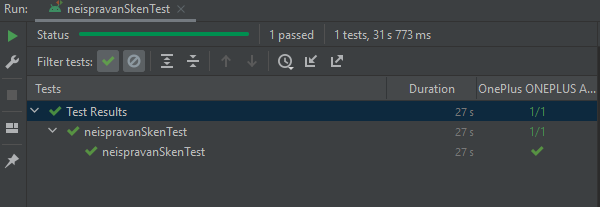
\includegraphics[scale=1]{./slike/test4.png}
	\caption{"Test neispravnosti skeniranog dokumenta"}
	\label{fig:test4}
\end{figure}\eject

Ako bi kojim slučajem skenirali traženi dokument, rezultat ne bi prošao test.

\begin{figure}[H]
	\centering
	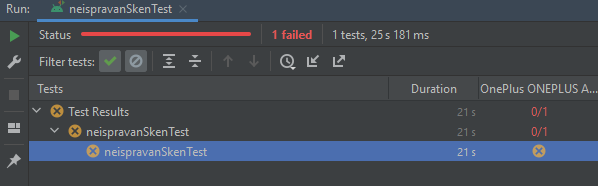
\includegraphics[scale=1]{./slike/test5.png}
	\caption{"Test neispravnosti skeniranog dokumenta"}
	\label{fig:test5}
\end{figure}\eject





	
		
		
		
		
		
		
			
			
			\eject 
		
		
	\section{Dijagram razmještaja}
	
	
	Klijent preko svojeg uređaja pristupa aplikaciji. Aplikacija se spaja na API Gateway koji je u sklopu Awsovog clouda. Unutar clouda se nalazi još virtualna mašina koja pokreće odgovarajuće lambda funkcije koje manipuliraju s bazom podataka koja je također dio clouda.
	
	\eject
	
	
	\begin{figure}
		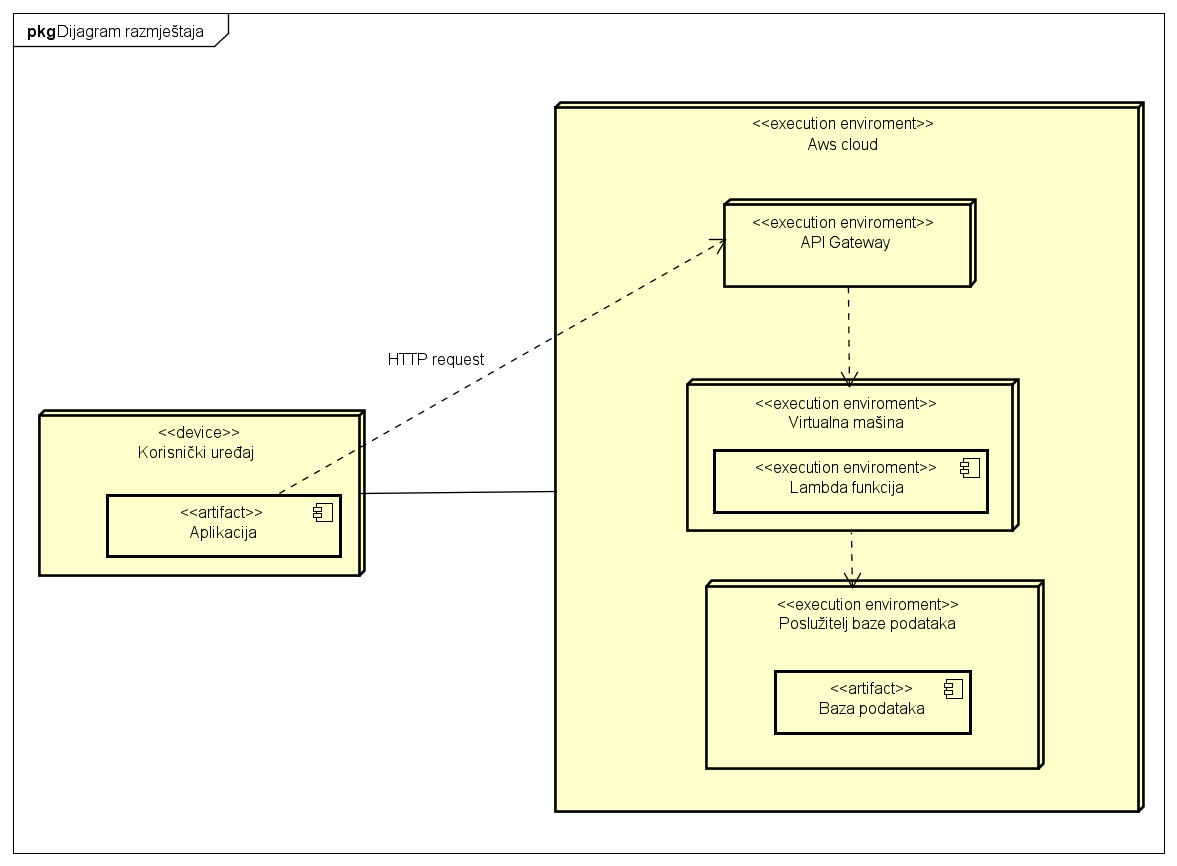
\includegraphics[width=\linewidth]{./dijagrami/dijagram_razmjestaja.png}
		\caption{Dijagram razmještaja}
		\label{fig:Raz}
	\end{figure}
	
	\eject
		
		\section{Upute za puštanje u pogon}
		
			\textbf{\textit{dio 2. revizije}}\\
		
		
			 
			 \subsection{Izgradnja aplikacije} 
			 
			 Kako bi se aplikacija izgradila, mora se prvo otvoriti u programu Android Studio, njezina putanja je :
			 \begin{itemize}
			 	\item  \path{is2-digitalizacija\IzvorniKod\Frontend\UI\SeptabilApp}.
			 \end{itemize}
			 
			\begin{figure}[H]
				\centering
				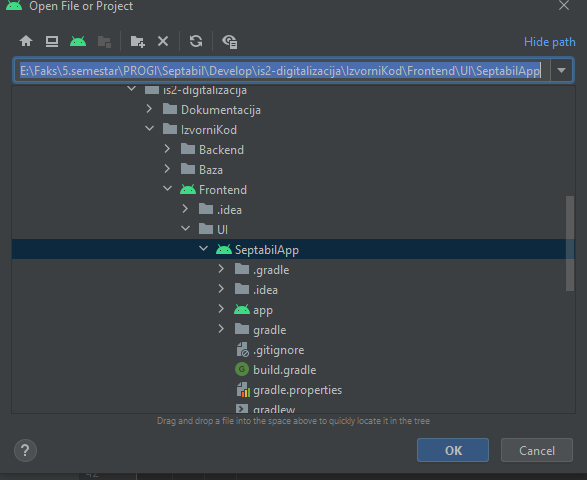
\includegraphics[scale=0.55]{./slike/astudio1.png}
				\caption{Android Studio - Path}
				\label{fig:astudio1}
			\end{figure}
		

			 Nakon što se aplikacija otvori, treba malo pričekati da Gradle učita sve potrebne pakete za rad i onda kada je sve učitano, korisnik treba kliknuti
			 \begin{itemize}
			  \item Build $\rightarrow$ Build Bundle(s) / APK(s) $\rightarrow$ Build APK \end{itemize}
			  kako bi napravio APK naše aplikacije.
			 \begin{figure}[H]
			 	\centering
			 	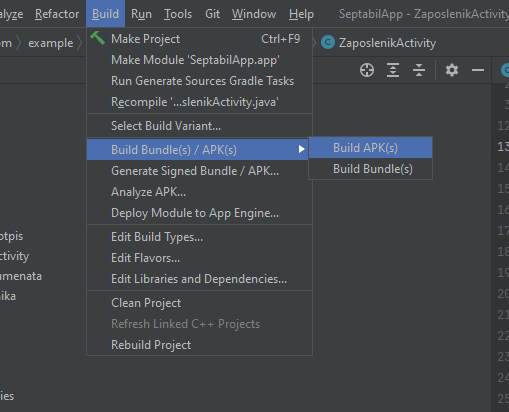
\includegraphics[scale=0.55]{./slike/astudio2.png}
			 	\caption{Android Studio - Build APK}
			 	\label{fig:astudio2}
			 \end{figure} 
			
			
			 \subsection{Postavljanje aplikacije na Amazon App trgovinu}  
			 Za postavljanje aplikacije na Amazon App trgovinu, prvo smo se morali registrirati na Amazon Developer.
			 Nakon toga treba odabrati
			 \begin{itemize}
			 	\item  Apps and Services $\rightarrow$ My apps
			 \end{itemize}
			 kliknuti gumb Add New App, 
			 odabrati želimo li mobilnu ili web aplikaciju i\\ upisati njezino ime.
		 	 \begin{figure}[H]
		 	 	\centering
		 	 	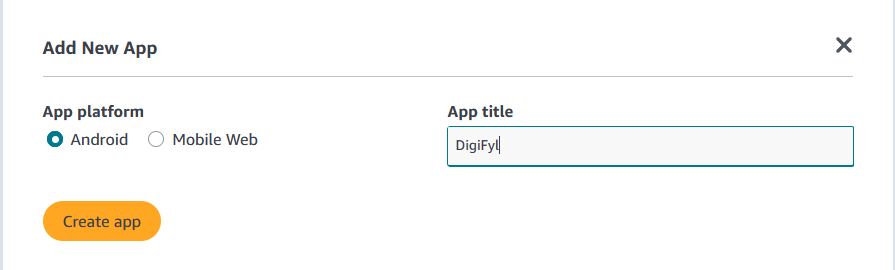
\includegraphics[scale=0.55]{./slike/amzn1.png}
		 	 	\caption{Amazon Developer - Add New App}
		 	 	\label{fig:amzn1}
		 	 \end{figure}
	 	 	\eject
	 	 	Kada odaberemo naziv aplikacije, otvorit će nam se prozor koji ima 6 dijelova za ispuniti, prvi dio su osnovne informacije o aplikaciji poput naslova, kategorije, kontakta...
	 	 	
	 	 	 \begin{figure}[H]
	 	 		\centering
	 	 		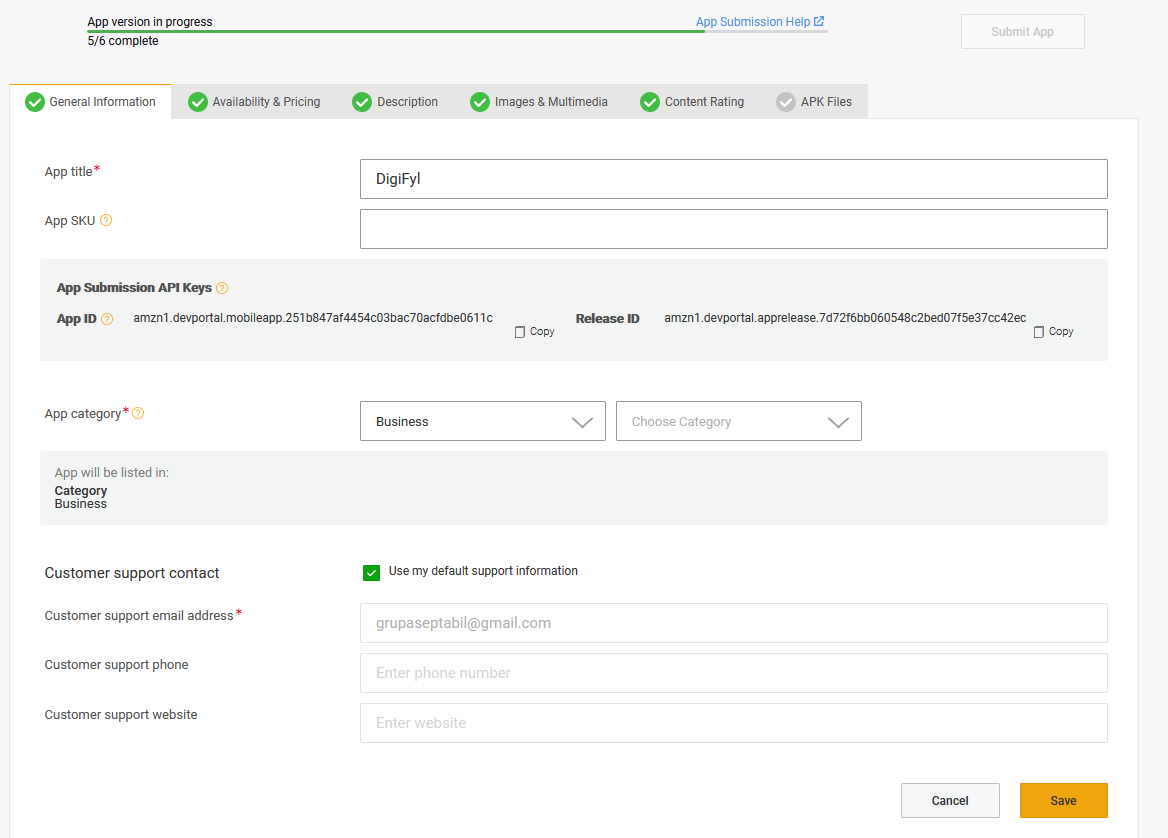
\includegraphics[scale=0.55]{./slike/amzn2.png}
	 	 		\caption{App - General Information}
	 	 		\label{fig:amzn2}
	 	 	\end{figure}
 	 	
 	 	Drugi dio nas samo pita gdje sve želimo da aplikacija bude dostupna u svijetu i želimo li ju izdati kao besplatnu ili naplaćivati.\eject
 	 	Treći dio je opis naše aplikacije, on će biti prikazan kao opis na Amazon App trgovini.
 	 		 \begin{figure}[H]
 	 		\centering
 	 		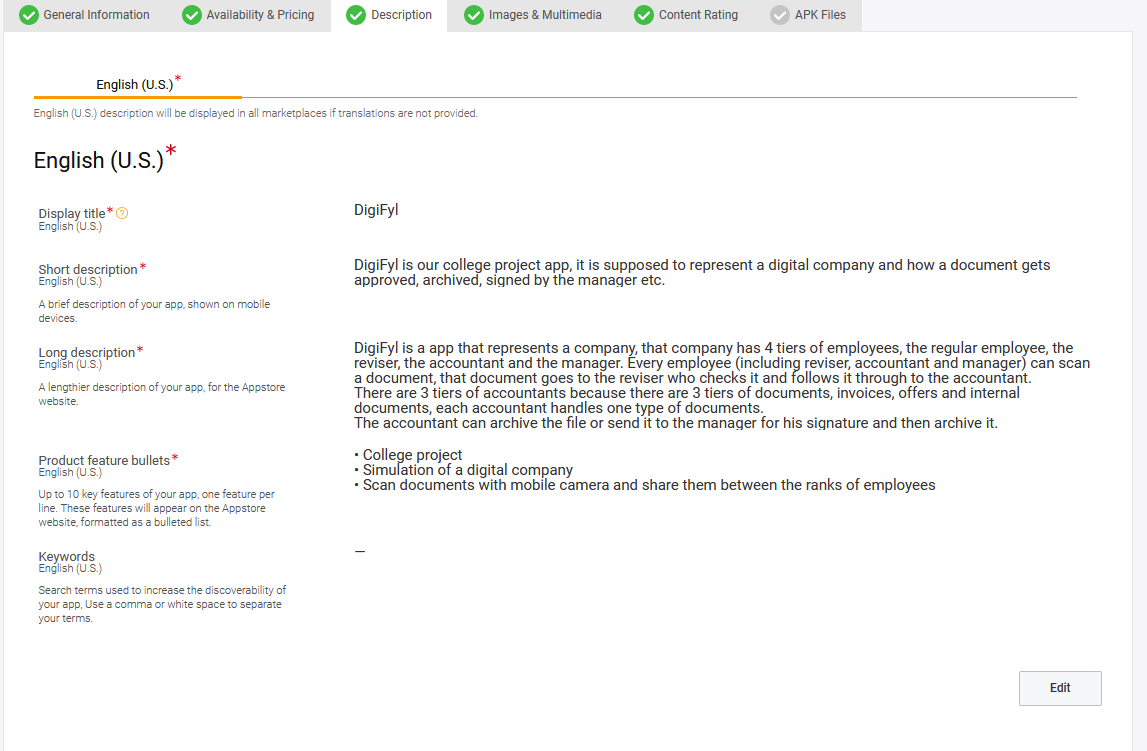
\includegraphics[scale=0.55]{./slike/amzn3.png}
 	 		\caption{App - Description}
 	 		\label{fig:amzn3}
 	 	\end{figure}
  	\eject
  	Četvrti dio od nas traži da postavimo ikonu aplikacije i priložimo 3-10 slika aplikacije, za ikonu smo u ovom slučaju koristili avion koji smo našli na stranici Icon Archive.
  	 \begin{figure}[H]
  		\centering
  		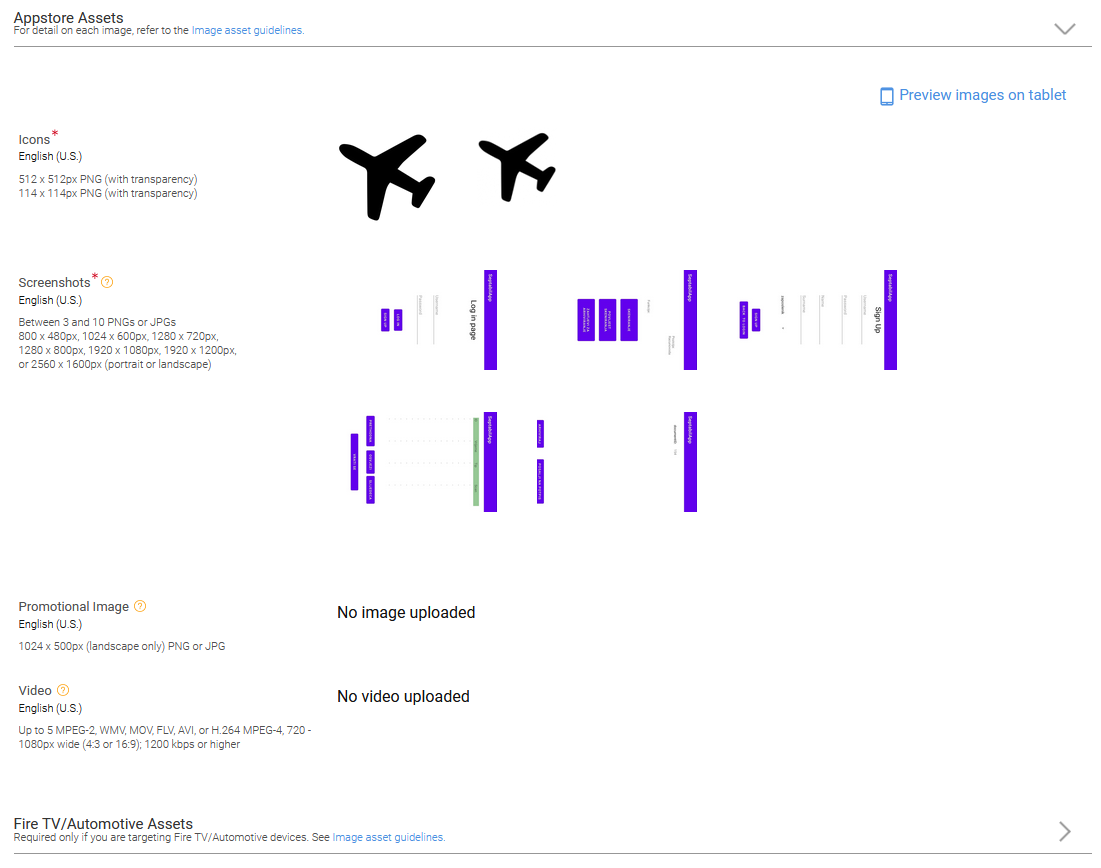
\includegraphics[scale=0.55]{./slike/amzn4.png}
  		\caption{App - Images and multimedia}
  		\label{fig:amzn4}
  	\end{figure} \eject
  
  U petom dijelu moramo napraviti "Content Rating" aplikacije, napisati ima li u njoj nasilja, netolerancije, je li ona u akademske svrhe ili ne...\\ Pita nas i da odaberemo ciljanu publiku te prikuplja li aplikacija osobne podatke. Zadnje stvari koje nas pita je ima li u aplikaciji reklama, kockanja, prikupljamo li lokacije korisnika i ima li komunikacije među korisnicima.\\
  Kako prikupljamo osobne podatke korisnika i oni mogu slati podatke jedni\\ drugima u obliku skeniranog dokumenta, to smo označili s da.
  	 \begin{figure}[H]
  	\centering
  	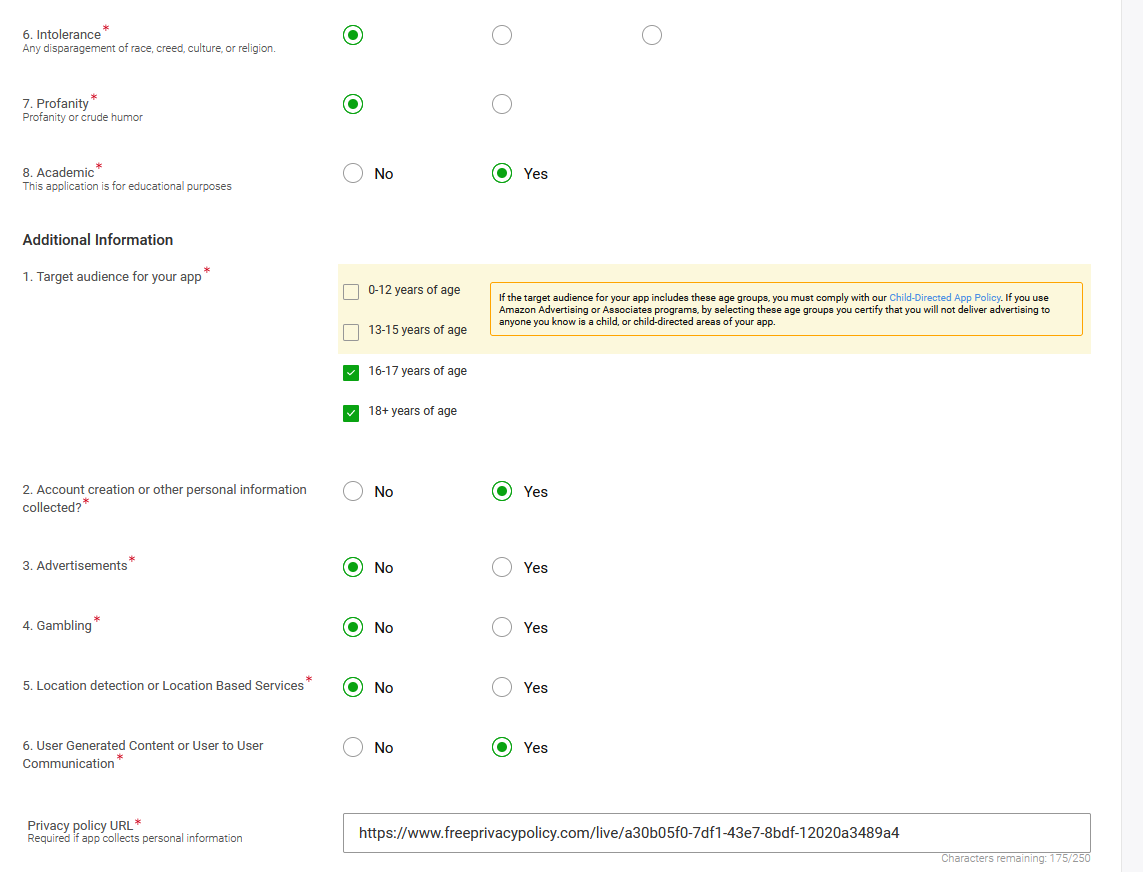
\includegraphics[scale=0.55]{./slike/amzn5.png}
  	\caption{App - Images and multimedia}
  	\label{fig:amzn5}
  \end{figure} 
  Na kraju, s obzirom na to da skupljamo podatke od korisnika, morali smo napraviti politiku privatnosti na kojoj piše koje sve podatke prikupljamo, kako ih koristimo i kako nas se može kontaktirati s bilo kojim dodatnim pitanjima.
  Priložit ćemo ju i ovdje:
  \href{https://www.freeprivacypolicy.com/live/a30b05f0-7df1-43e7-8bdf-12020a3489a4}{\underline{link}}\eject
  	
  	Zadnji dio u deployanju naše aplikacije je odabrati APK datoteku koju\\ predajemo, podržane jezike aplikacije i dodatno napisati upute za testiranje ako će trebati Amazonovom timu, a moramo i odabrati da smo suglasni da se aplikacija uvozi i izvozi iz SAD-a u druge države u kojima Amazon radi.
  		 \begin{figure}[H]
  		\centering
  		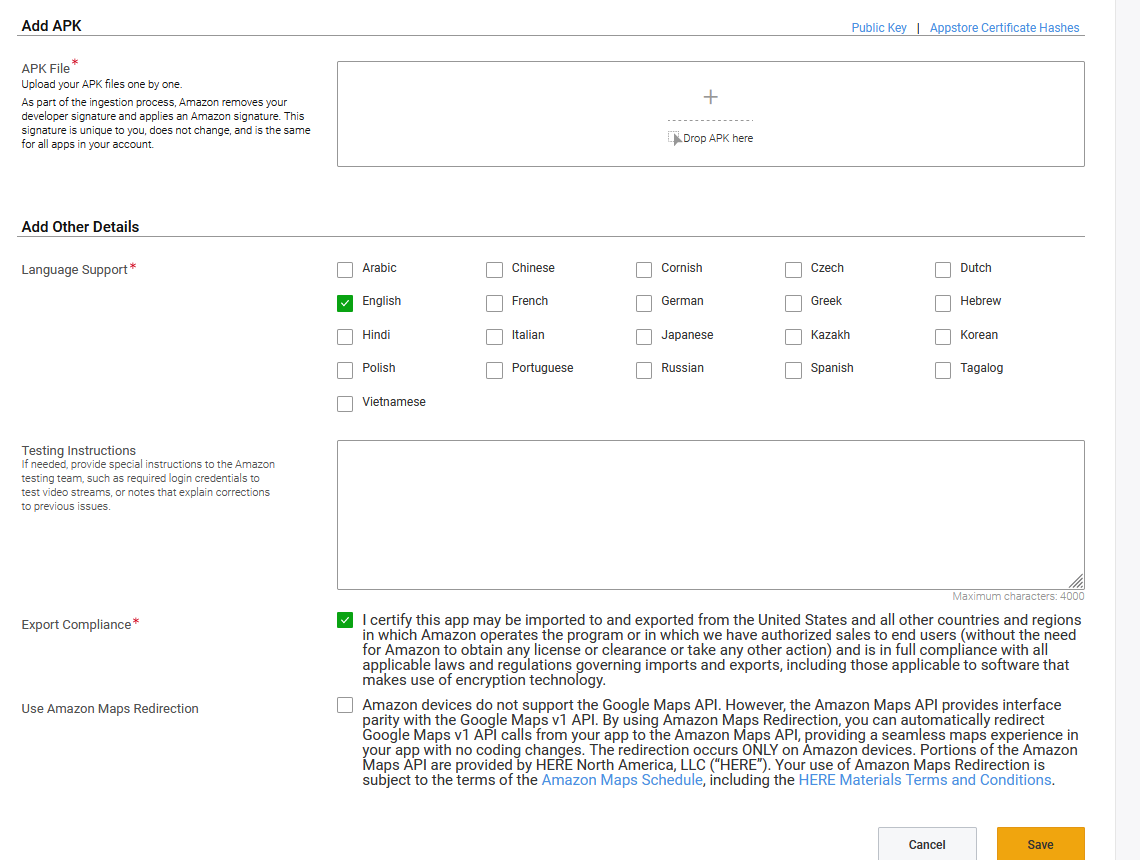
\includegraphics[scale=0.55]{./slike/amzn6.png}
  		\caption{App - APK Files}
  		\label{fig:amzn6}
  	\end{figure} \eject
  
  \subsection{Postavljanje baze podataka na Amazon RDS-u}
 
 Kako bi postavili bazu podataka, morali smo otići na Amazon RDS, odabrati "Databases" i kliknuti "Create Database".\\
 Tad nam se prikaže izbornik koji nas pita za vrstu baze podataka, mi smo radili s postgreSQL bazom.
 	 \begin{figure}[H]
 	\centering
 	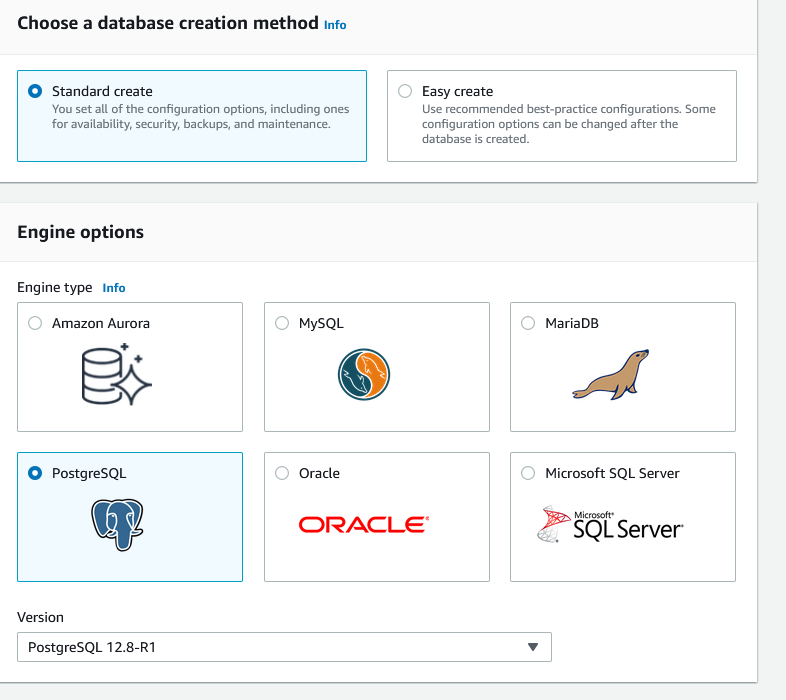
\includegraphics[scale=0.55]{./slike/rds1.png}
 	\caption{Amazon RDS - DB Setup}
 	\label{fig:rds1}
 \end{figure}\eject

Nakon odabira baze podataka, RDS traži da upišemo ime instance baze\\ podataka te da joj priložimo korisničko ime i lozinku kojom će joj se pristupati.
	 \begin{figure}[H]
	\centering
	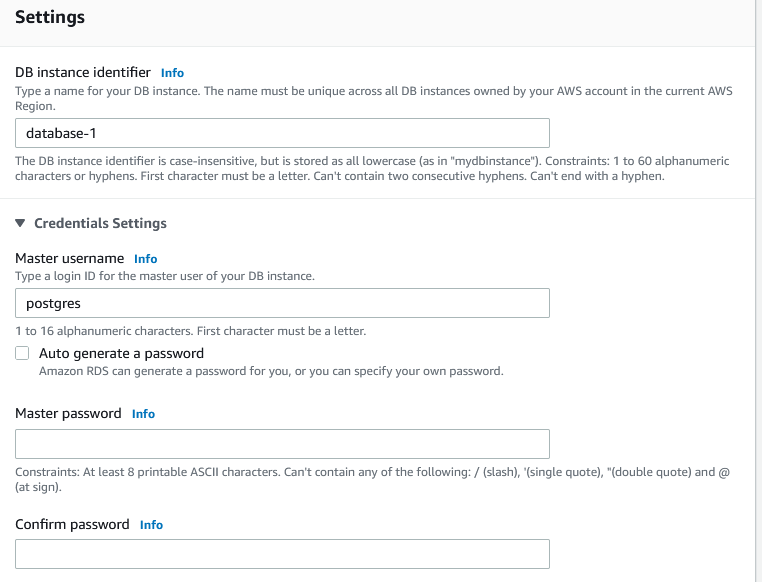
\includegraphics[scale=0.55]{./slike/rds2.png}
	\caption{Amazon RDS - DB Instance}
	\label{fig:rds2}
\end{figure}

Sljedeće što nas RDS pita je koliko nam memorije treba za bazu, minimalan odabir je 20 GB, a nama ni ne treba više pa smo odabrali to, ali smo upalili\\ automatsko skaliranje skladišta, dakle ako nam treba više od 20 GB u nekom\\ trenutku, dobit ćemo tu memoriju.
	 \begin{figure}[H]
	\centering
	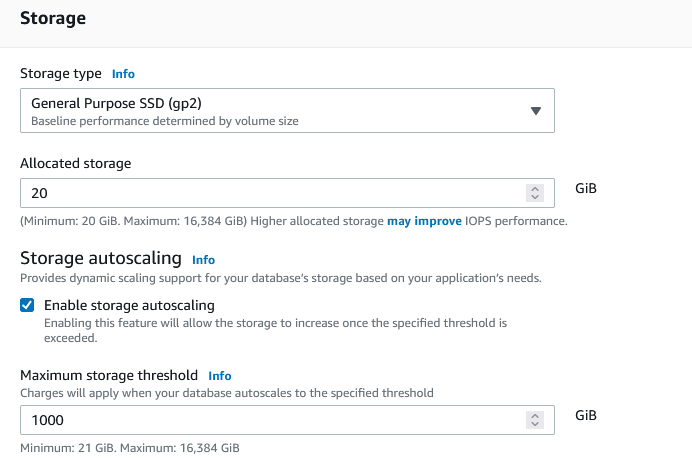
\includegraphics[scale=0.55]{./slike/rds3.png}
	\caption{Amazon RDS - DB Storage}
	\label{fig:rds3}
\end{figure}\eject

Sljedeći obrazac se tiče povezivosti, stvaramo virtualni oblak za našu bazu i grupu podmreža koje baza može koristiti (što smo postavili na sve), također\\ postavljamo i javni pristup našoj bazi kako bi joj mogli pristupiti iz pgAdmin-a.
	 \begin{figure}[H]
	\centering
	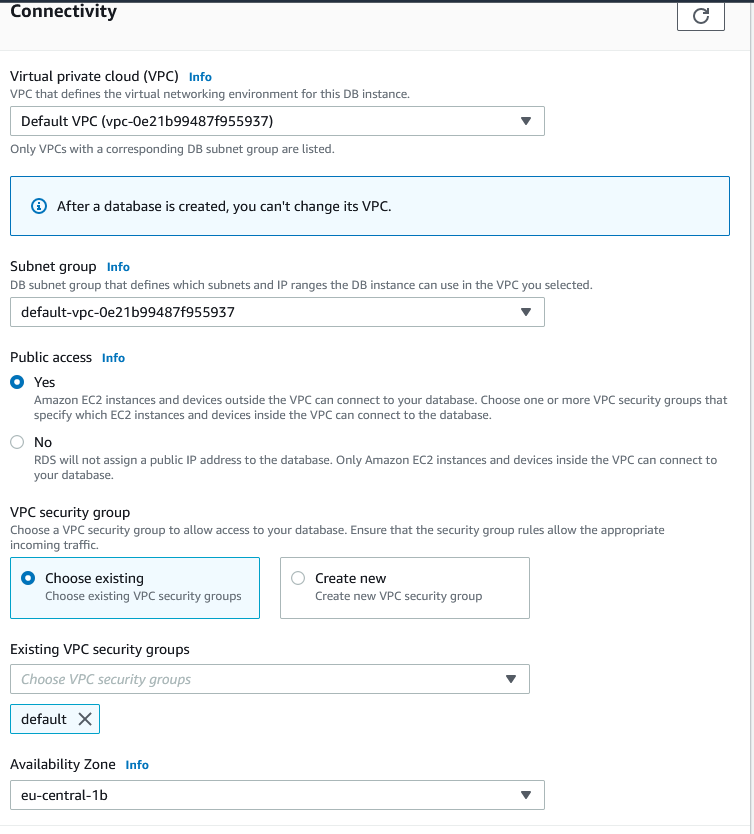
\includegraphics[scale=0.55]{./slike/rds4.png}
	\caption{Amazon RDS - Connectivity}
	\label{fig:rds4}
\end{figure}\eject

Zadnji obrazac nas pita za ime baze podataka i vrijeme zadržavanja sigurnosnih kopija prije brisanja.

	 \begin{figure}[H]
	\centering
	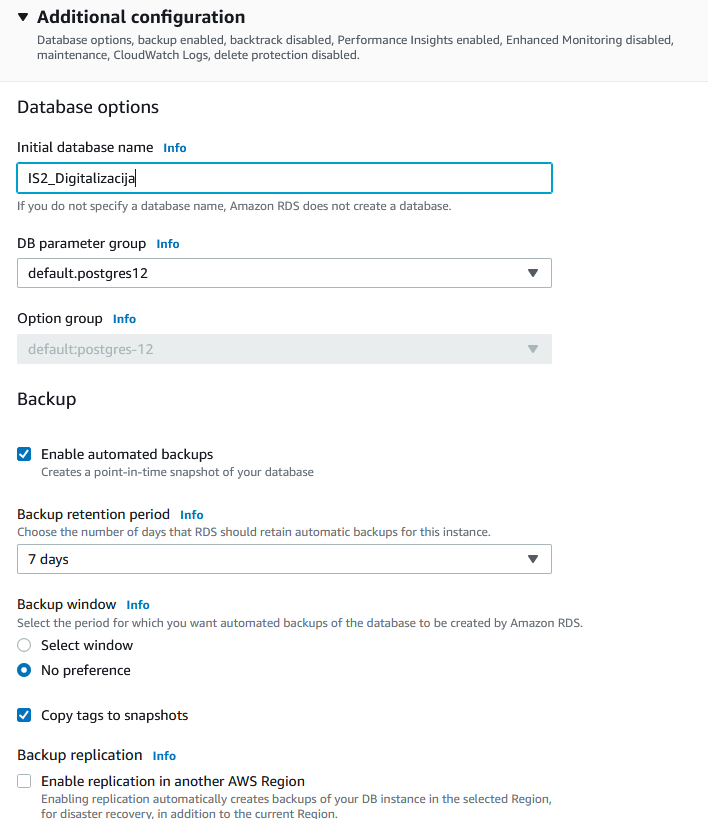
\includegraphics[scale=0.55]{./slike/rds5.png}
	\caption{Amazon RDS - DB Name and Backup}
	\label{fig:rds5}
\end{figure}\eject

Nakon što stvorimo bazu na Amazon RDS-u, dobijemo krajnju točku kako bi se na bazu mogli spojiti iz pgAdmin-a i Python-a. Za spajanje nam trebaju i\\ korisničko ime i lozinka, ali to smo postavili pri stvaranju baze.
	 \begin{figure}[H]
	\centering
	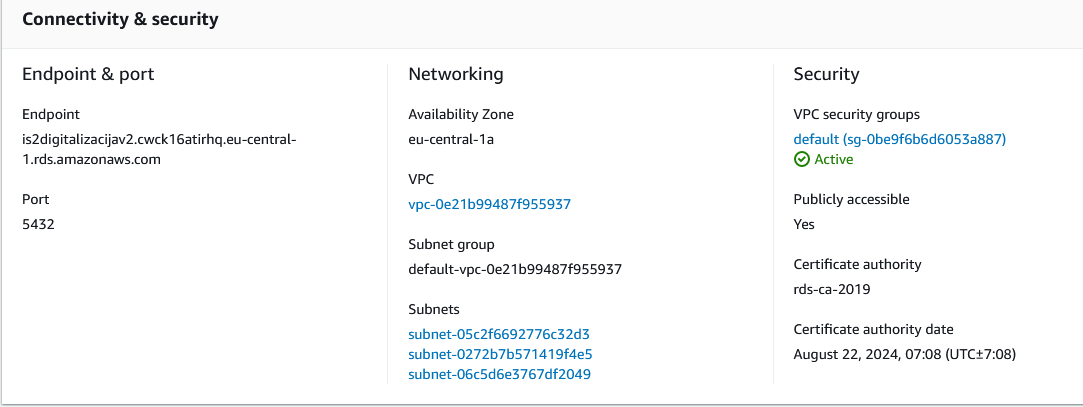
\includegraphics[scale=0.55]{./slike/rds6.png}
	\caption{Amazon RDS - DB Endpoint}
	\label{fig:rds6}
\end{figure}





 
	 	 	 
		 	 
			\eject 
			